\chapter{Estudios del Cotransportador vSGLT}
\section{Introducci\'{o}n}
El presente estudio se ocupa de una prote\'{i}na encontrada en la membrana de la bacteria \textit{Vibrio Parahaemoliticus}. Pero antes de realizar dicho estudio es necesario conocer las siguientes preguntas fundamentales: ?`qu\'{e} es una prote\'{i}na? ?`de qu\'{e} est\'{a} conformada una prote\'{i}na? ?`d\'{o}nde se encuentran las prote\'{i}nas? ?`cu\'{a}l es el papel que desempe\~{n}an las prote\'{i}nas en los seres vivos? ?`Cu\'{a}l es la forma de las prote\'{i}nas?.\\ \\

Una prote\'{i}na es un pol\'{i}mero (pol\'{i}- Muchas -mero: Partes) que est\'{a} formado por una gran cantidad de unidades del mismo tipo, estas unidades se conocen como amino\'{a}cidos. Espec\'{i}ficamente se dice que las prote\'{i}nas son polip\'{e}ptidos \footnote{P\'{e}ptido: Mol\'{e}cula formada por una cadena de varios amino\'{a}cidos mediante un enlace llamado pept\'{i}dico; normalmente se le dice pept\'{i}do a una cadena con menos de $20\sim30$  amino\'{a}cidos} que tienen m\'{a}s de 50 amino\'{a}cidos, haciendo que su peso molecular sea mayor a 5000 Da \cite{Kuchel}.\\

Un amino\'{a}cido es una mol\'{e}cula org\'{a}nica formada por un carbono llamado $\alpha$ alrededor del cual se encuentran los grupos funcionales carboxilo y amino, adem\'{a}s de un hidr\'{o}geno y un radical que le da la identidad a cada amino\'{a}cido, ver figura \ref{fig:amino}.\\
\begin{figure}[H]
\centering
\chemfig{C^{\alpha}(-[:0]H)(-[:90]COO^{-})(-[:180]NH_{3}^{+})(-[:270]R)}
\caption{Forma general de un L-amino\'{a}cido a pH 7. El radical \ce{R} cambia para cada amino\'{a}cido.}\label{fig:amino}
\end{figure}
A continuaci\'{o}n se muestran los 20 amino\'{a}cidos proteinog\'{e}nicos  comunes \footnote{Son los incorporados en la s\'{i}ntesis de prote\'{i}nas durante la traducci\'{o}n en el ribosoma}  clasificados de acuerdo a la carga, la polaridad y la formaci\'{o}n de grupos arom\'{a}ticos. Las abreviaciones de los amino\'{a}cidos se encuentran en la lista de s\'{i}mbolos.\\
\begin{figure}[h]
\begin{center}
\begin{picture}(100,100)
\put(0,60){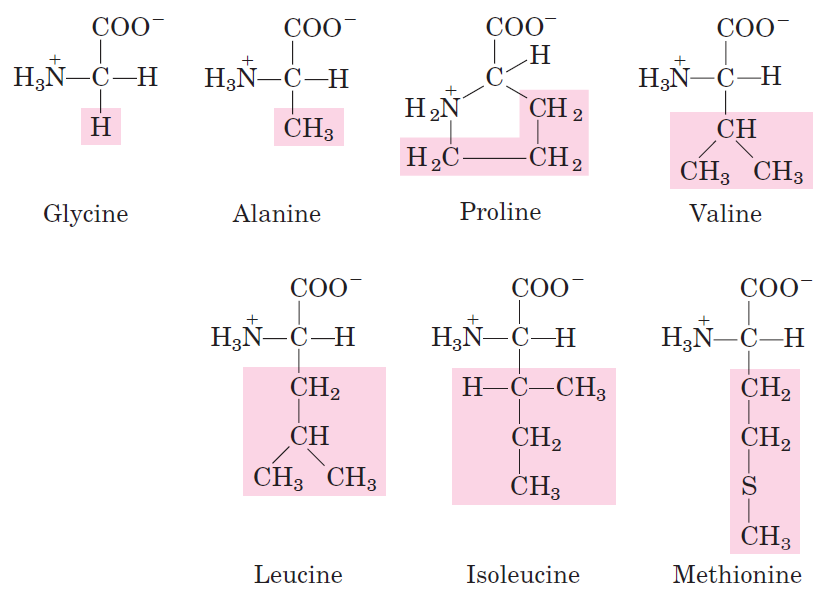
\includegraphics[scale=0.3]{Kap2/nopolar.png}}
\put(70,75){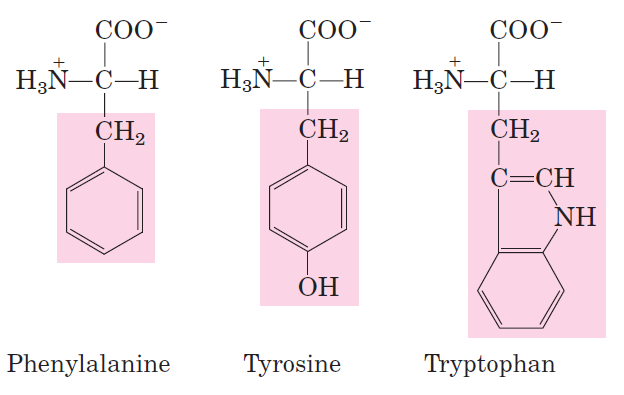
\includegraphics[scale=0.3]{Kap2/aromatico.png}}
\put(0,0){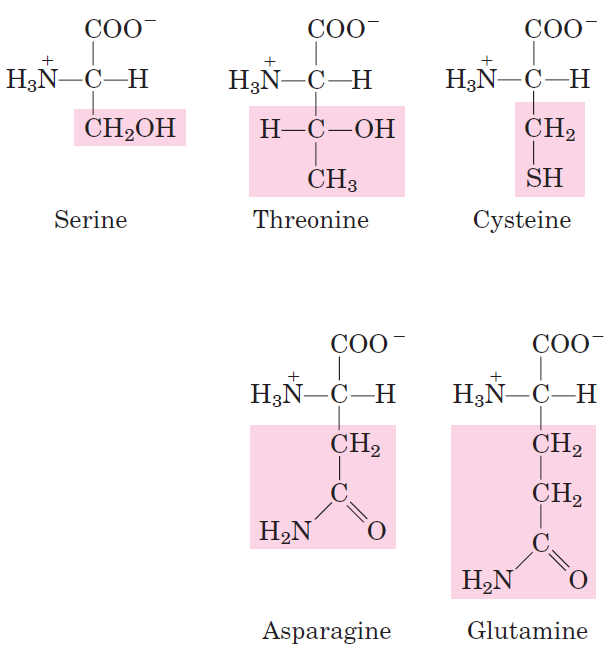
\includegraphics[scale=0.3]{Kap2/polardescargado.png}}
\put(70,30){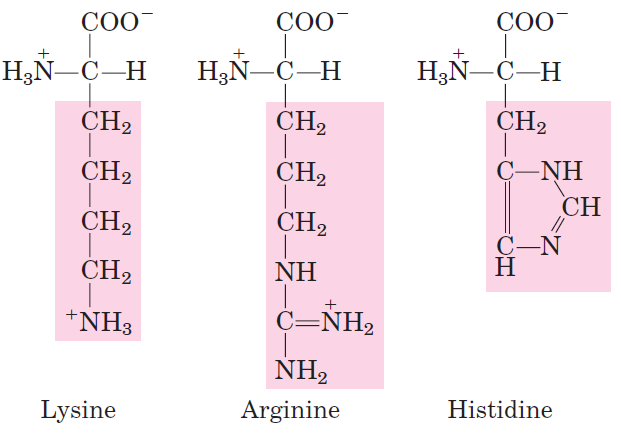
\includegraphics[scale=0.3]{Kap2/qpp.png}}
\put(70,-5){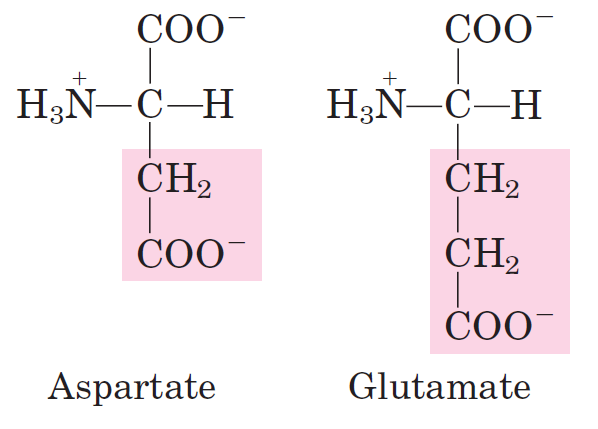
\includegraphics[scale=0.2]{Kap2/qmm.png}}
\put(0,110){No polar, grupo R alif\'{a}tico}
\put(70,110){Grupo R arom\'{a}tico}
\put(0,55){Polar descargado}
\put(70,65){Grupo R cargado positivamente}
\put(70,20){Grupo R cargado negativamente}
\end{picture}
 \end{center}
\caption{F\'{o}rmulas estructurales de los 20 amino\'{a}cidos proteinog\'{e}nicos a pH 7 clasificados seg\'{u}n su radical de color rosado. Tomado de \cite{Nelson2011}.}
\end{figure}

Exceptuando la glicina, todos los amino\'{a}cidos presentan la propiedad de la quiralidad, existiendo dos posibles formas posibles para cada amino\'{a}cido: L-amino\'{a}cidos o D-amino\'{a}cidos. La distinci\'{o}n va eg\'{u}n la direcci\'{o}n en la que desv\'{i}en la luz con respecto al centro quiral que es el C-$\alpha$ del amino\'{a}cido.  Pr\'{a}cticamente todos los amino\'{a}cidos encontrados en prote\'{i}nas tienen la forma L.
\section{Formaci\'{o}n de P\'{e}ptidos y Prote\'{i}nas}
Dos amino\'{a}cidos reaccionan formando un enlace llamado pept\'{i}dico, esto ocurre cuando el carbono del grupo carboxilo se enlaza covalentemente con el nitr\'{o}geno del grupo amino, liberando de la reacci\'{o}n agua. En la figura se muestra los reactantes y los productos de la reacci\'{o}n.
\begin{figure}[H]
\centering
\chemfig{C^{\alpha}(-[:0]H)(-[:90]COO^{-})(-[:180]NH_{3}^{+})(-[:270]R)}
\caption{Forma general de un L-amino\'{a}cido a pH 7. El radical \ce{R} cambia para cada amino\'{a}cido.}\label{fig:pepti}
\end{figure}
\section{Prote\'{i}nas de Membrana}

\section{Transportadores}
La membrana celular al ser hidrof\'{o}bica permite protegerse de la regi\'{o}n extracelular, sin embargo, ella necesita ingresar y expulsar todos los compuestos necesarios para realizar su fisiolog\'{i}a OJO. La membranana celular tiene prote\'{i}nas que permiten el ingreso y la expulsi\'{o}n de estos compuestos. Entre los tipos de prote\'{i}nas se encuentran  los poros, las bombas, los transportadores y los canales. \\

Los transportadores se clasifican, de acuerdo al sistema de clasificaci\'{o}n de transportadores \cite{Nelson2011}, en dos categor\'{i}as principales de las cuales se desprenden otras subcategor\'{i}as :
\begin{enumerate}
 \item \textbf{Portadores}:
 \begin{enumerate}
 \item[1.] Transportadores activos primarios
 \item[2.a] Transportadores activos secundarios
  \begin{enumerate}
 \item[a)] Simportadores
 \item[b)] Antiportadores
 \end{enumerate}
 \item[2.b] Uniportadores
 \end{enumerate}
 \item  \textbf{Canales i\'{o}nicos}: Los canales se diferencian de los portadores en la raz\'{o}n a la que transportan los iones, que es de $10^6$ iones/segundo  (muy alta) as\'{i} como en que los canales no necesitan energ\'{i}a metab\'{o}lica para transportar los iones.
\end{enumerate}


Para visualizar las prote\'{i}nas se puede usar el microscopio de fuerza at\'{o}mico
\subsection{Cotransportadores}
Hacia la d\'{e}cada de los a\~{n}os sesenta Robert Crane, ver \cite{Hamilton2013}, estableci\'{o} una relaci\'{o}n acoplada o de \textit{cotransporte} entre el ion de sodio y la glucosa los cuales son absorbidos por el intestino delgado. El conocimiento de este mecanismo ha permitido realizar el tratamiento de la diarrea y del c\'{o}lera mediante la rehidrataci\'{o}n oral. La hip\'{o}tesis del cotransporte que ha sido numerosamente validada y ha sido una piedra angular para el entendimiento de el metabolismo de los carbohidratos, claves en la energ\'{e}tica celular. La hip\'{o}tesis del cotransporte tambi\'{e}n se ha extendido a otros organismos vivos, con la diferencia de que el acoplamiento del sodio se puede dar con cualquier otro soluto org\'{a}nico \cite{Faham2008}.\\
\section{Algunas Familias Proteicas y enrollamiento LeuT (LeuT fold)}
\section{Co-transportador vSGLT}
El cotransportador de Na+/Galactosa presente en la proteobacteria \textit{Vibrio Parahaemolyticus } denotado como vSGLT, es un simportador perteneciente a la familia de simportadores de $\mathrm{Na}^+$-soluto SSS \cite{SaierJr.quotTheFamilyquot}.\\
La caracterizaci\'{o}n molecular del compuesto se realiz\'{o} por primera vez hacia el a\~{n}o 2000 ver \cite{Turk2000}, mientras que la determinaci\'{o}n de su estructura fue posible hacia el a\~{n}o 2008 \cite{Faham2008}. En dichos estudios se establece que vSGLT es similar en la estructura primaria y terciaria a otros transportadores de la familia SLC5 como por ejemplo NIS, SGLT1, SGLT2.
\section{Estudios actuales del Co-transportador vSGLT}
